\documentclass{beamer}
\usepackage[spanish]{babel}
\usepackage[T1]{fontenc}
\usepackage[utf8]{inputenc}
\usetheme{Boadilla}
\usefonttheme{structuresmallcapsserif}
\usecolortheme{beaver}
\usepackage[normalem]{ulem}
\usepackage{enumitem}
\usepackage{parskip}
\setlength{\parskip}{7pt}

% == To show Python code ==
%\usepackage{listings}
\usepackage{listingsutf8}
\usepackage{xcolor}

\usepackage[table]{xcolor}


\definecolor{codegray}{gray}{0.95}
\definecolor{keywordcolor}{rgb}{0.2, 0.2, 0.7}
\definecolor{commentcolor}{rgb}{0.0, 0.5, 0.0}
\definecolor{stringcolor}{rgb}{0.58, 0, 0.82}
\definecolor{backcolor}{rgb}{0.97, 0.97, 0.97}

\definecolor{codegray}{gray}{0.95}

\lstdefinestyle{mystyle}{
    language=Python,
    backgroundcolor=\color{codegray},
    basicstyle=\ttfamily\footnotesize,
    keywordstyle=\color{keywordcolor}\bfseries,
    commentstyle=\color{commentcolor}\itshape,
    stringstyle=\color{stringcolor},
    breaklines=true,
    frame=single,
    showstringspaces=false,
    numbers=left,
    numberstyle=\tiny\color{black},
    stepnumber=1,
    tabsize=4    
}

\lstset{style=mystyle}
% ====================================

\usepackage{pifont}
\usepackage{graphicx}
\usepackage{gb4e}
\usepackage{array}
\usepackage{hyperref}

\resetcounteronoverlays{exx} %So  does not affect numbering
\let\eachwordone=\sffamily
\let\eachwordtwo=\sffamily
\usepackage[figurename={}]{caption}
%\usepackage[bottom]{footmisc}
\expandafter\def\expandafter\quote\expandafter{\quote\small} %smaller font in quotes
\newcommand{\downbracketlabel}[2] {$\underbrace{\textrm{#1}}_{\textrm{#2}}$} %low curvy brackets
\newcommand{\corchete}[2] {$\underbracket{\textrm{#1}}_{\textrm{\textsuperscript{#2}}}$} %straight brackets
\newcommand{\blue}[1] {{\color{blue} #1}}

%\noautomath


\title[Datos y aplicación]{Datos, análisis y aplicación}

\institute[]{}

\date[Día 3]{\footnotesize\texttt{Introducción al Procesamiento del Lenguaje Natural con Python e IA}\\ \vspace{10pt} Tercer encuentro}

\author[C. Mu\~{n}oz P\'{e}rez]{Carlos Mu\~{n}oz P\'{e}rez}

\begin{document}
	\frame{\titlepage}
	

\begin{frame}
\frametitle{Introducción}

En este encuentro, veremos una puesta en práctica integral de los conocimientos básicos de \alert{\textit{Python}} que adquirieron en los días previos.

\begin{itemize}
\item[\ding{229}] Exploraremos un proyecto que llevé a cabo hace un par de años y que tiene un cierto grado de aplicabilidad en el mundo real.
\end{itemize}


Esto nos servirá de excusa para abordar tres puntos importantes en el proceso de desarrollo de herramientas de \alert{\textit{aprendizaje automático}}.


\begin{enumerate}
\item La obtención de \alert{\textit{datos}} para entrenar nuestros modelos


\item El \alert{\textit{análisis}} de dichos datos (que puede ser relevante especialmente en contextos académicos)


\item El \alert{\textit{entrenamiento}} de un modelo y su \alert{\textit{implementación}} para que pueda realizar inferencias en la práctica
\end{enumerate}


\end{frame}


\begin{frame}
\frametitle{LingPeer}

Escenario:

\vspace{10pt}

\begin{quote}
Son miembros del comité editorial de una revista académica de lingüística. Les llega un nuevo manuscrito acerca de algún tema oscuro de gramática. ¿Cómo elegirían a los revisores para ese artículo? ¿Contactarían a algún conocido? ¿Buscarían en Google? ¿Se fijarían quién revisó artículos similares para la revista en el pasado? Cualquiera sea la respuesta, descubrirán que encontrar revisores adecuados es un proceso que toma tiempo.
\end{quote}

\end{frame}


\begin{frame}
\frametitle{LingPeer}

Teniendo este tipo de escenario en mente, desarrollé \href{https://lingpeer.streamlit.app/}{\alert{\textit{LingPeer}}}.


\begin{itemize}
\item[\ding{52}] \href{https://lingpeer.streamlit.app/}{\alert{\textit{LingPeer}}} es una aplicación que sugiere revisores para manuscritos en lingüística teórica.

\item[\ding{52}] Utiliza datos de \href{https://ling.auf.net/lingbuzz/lingbuzz}{\alert{\textit{Lingbuzz}}}, un repositorio en línea de manuscritos en lingüística, para identificar expertos relevantes de forma automática.

\item[\ding{52}] Está disponible como aplicación web; solo se necesitan (i) el título del artículo, (ii) sus palabras clave y (iii) el resumen.

\end{itemize}

\end{frame}

\begin{frame}
\frametitle{LingPeer}

Veamos cómo funciona \href{https://lingpeer.streamlit.app/}{\alert{\textit{LingPeer}}}.

\end{frame}



\begin{frame}
\frametitle{Extracción de datos}

Los datos a partir de los cuales se entrenó \alert{\textit{LingPeer}} se tomaron de \alert{\textit{Lingbuzz}}.

\begin{itemize}
\item[\ding{229}] \alert{\textit{Lingbuzz}} es un repositorio en línea de acceso abierto que se especializa en trabajos académicos de lingüística teórica.

\item[\ding{229}] Permite a los investigadores subir manuscritos, artículos, y libros, incluso si aún no se han publicado.

\item[\ding{229}] Aunque no tiene el status de una revista especializada, LingBuzz ha ganado prestigio como archivo y fuente de consulta dentro de la comunidad lingüística.

\item[\ding{229}] La plataforma es gestionada por Michal Starke.

\end{itemize}


\end{frame}

\begin{frame}
\frametitle{Extracción de datos}

Visitemos \href{https://ling.auf.net/lingbuzz/lingbuzz}{\alert{\textit{Lingbuzz}}} y analicemos brevemente su código.

\end{frame}



\begin{frame}
\frametitle{Extracción de datos}

El \alert{\textit{web scraping}} es una técnica para extraer información de sitios web de forma automática.

\begin{itemize}
\item[\ding{52}] Se usan scripts o u otras herramientas que simulan la navegación web y recuperan contenido de páginas HTML.
\end{itemize}


La extracción de datos suele seguir los siguientes pasos.

\begin{enumerate}
\item Se realiza una solicitud a la página web.

\item Se recibe como respuesta la información contenida en la página web.

\item El programa (\textit{\alert{scraper}}) analiza la estructura de la página web.

\item Se extraen y guardan los datos relevantes (texto, imágenes, links, etc.).
\end{enumerate}

\end{frame}

\begin{frame}
\frametitle{Extracción de datos}

El \alert{\textit{scraping}} debe hacerse de manera responsable y ética. Por lo general, se dice que hay que seguir una cierta ``etiqueta''.

\begin{itemize}
\item[\ding{52}] Las páginas tienen tienen un archivo llamado \texttt{\blue{robots.txt}} que especifica qué tipo de scraping se puede realizar.

\item[\ding{52}] Hay que evitar sobrecargar los servidores: hay que espaciar la frecuencia de las solicitudes, e.g., 3 segundos entre consultas.

\item[\ding{52}] En mi caso, pedí permiso para tomar los datos de \alert{\textit{Lingbuzz}}, e incorporé un mecanismo de delay en el \alert{\textit{scraper}}.
\end{itemize}

Si no respetan estas condiciones, pueden banear su IP del sitio web, e incluso podría haber consecuencias legales.

\end{frame}

\begin{frame}
\frametitle{Extracción de datos}

Veamos algunos aspectos básicos de \alert{\textit{web scraping}}.


\begin{itemize}
\item[\ding{229}] \href{https://colab.research.google.com/drive/1N2M1gnpTMQAwDwskLtsPl0keQ-OzNXdp?usp=sharing}{\blue{\textit{\uline{Notebook 1: web scraping con Python}}}}
\end{itemize}

\end{frame}

\begin{frame}
\frametitle{Exploración de los datos}

Antes de aplicar modelos predictivos o de aprendizaje automático, se recomienda realizar un \alert{\textit{análisis exploratorio de los datos}} (EDA).

\begin{itemize}
\item[\ding{52}] El objetivo general del EDA es familiarizarse con los datos a utilizar.

\item[\ding{52}] Esto involucra detectar tendencias en los datos, evaluar su calidad y formular generalizaciones sobre su comportamiento.

\end{itemize}

Vamos a hacer un breve análisis de la información obtenida a partir de \alert{\textit{scraping}}.

\begin{itemize}
\item[\ding{229}] Además, vamos a usar la oportunidad como excusa para mostrar algunas herramientas de Python para el análisis ed datos.
\end{itemize}

\end{frame}

\begin{frame}
\frametitle{Exploración de los datos}

\begin{itemize}
\item[\ding{229}] \href{https://colab.research.google.com/drive/1yxesc-NQFy2TI05ux38Xbt5SduvjETlw?usp=sharing}{\blue{\textit{\uline{Notebook 2: exploración de datos con Python}}}}
\end{itemize}

\end{frame}

\begin{frame}
\frametitle{Multinomial naive Bayes classifier}

\alert{\textit{LingPeer}} se basa en un ensamble de dos clasificadores \alert{\textit{naive Bayes}}.

\begin{itemize}
\item[\ding{229}] Cuando el programa sugiere un revisor, lo que en realidad está haciendo es intentar predecir el autor del abstract.
\item[\ding{229}] Lo que hice fue tomar las predicciones de dos modelos entrenados con diferentes reordenamientos de los datos y seleccionar los potenciales autores a partir de un cierto margen de certeza.
\end{itemize}

¿Es esta una metodología adecuada?

\vspace{10pt}

\begin{quote}
\blue{-- No sé, pero más o menos funciona.}
\end{quote}

\end{frame}

\begin{frame}
\frametitle{Multinomial naive Bayes classifier}

\begin{center}

\includegraphics[scale=0.24]{ml.png}
\end{center}

\end{frame}




\begin{frame}
\frametitle{Multinomial naive Bayes classifier}
Supongan que tenemos los siguientes datos (ejemplo de \href{https://youtu.be/O2L2Uv9pdDA?si=2F0ZbvJCi7qTbQ8u}{\alert{\textit{Statquest}}}).

\begin{center}
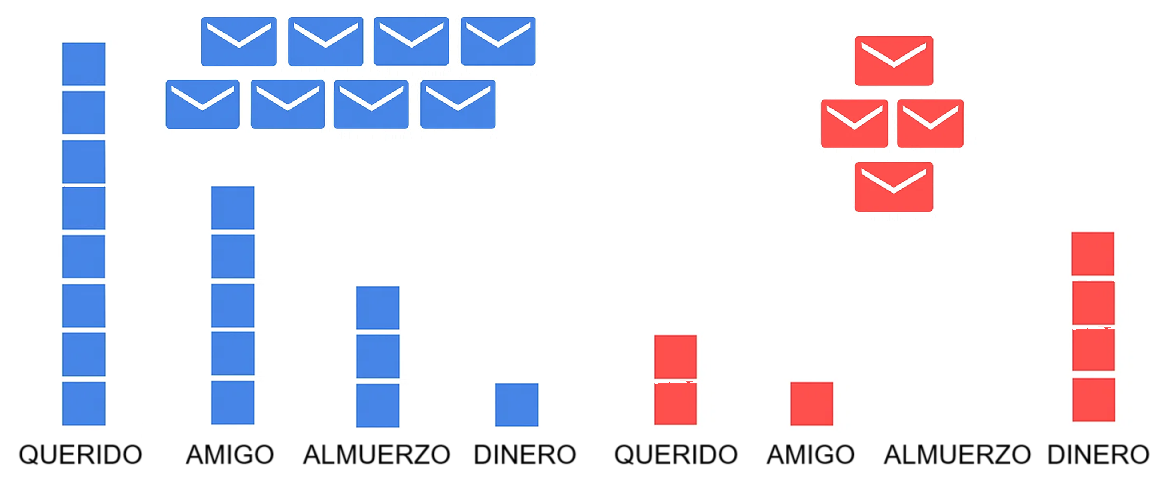
\includegraphics[scale=0.35]{bayes.png}
\end{center}

Esto permite predecir si el correo \textbf{\textit{`querido amigo'}} es \blue{\textit{deseado}} o \alert{\textit{spam}}.

\vspace{-5pt}

\begin{exe}
\sn{\blue{8/12 x 8/17 x 5/17 = 0.67 x 0.47 x 0.29 = 0.09}}
\sn{\alert{4/12 x 2/7 x 1/7 = 0.33 x 0.29 x 0.14 = 0.01}}
\end{exe}
\vspace{-5pt}
Resultado: \blue{\textit{querido amigo}} no es spam porque \blue{0.09} > \alert{0.01}.

\vspace{10pt}

\end{frame}

\begin{frame}
\frametitle{Preprocesamiento}

\begin{itemize}
    \item \alert{\textit{Unificación del texto:}} se combinan el \textit{título} y el \textit{resumen} (abstract) en un solo campo.
    \item \alert{\textit{Lematización:}} se reduce cada palabra a su forma ``de diccionario'' para facilitar la detección de similitudes semánticas.
    \item \alert{\textit{Balance de etiquetas:}} se normaliza el conjunto de entrenamiento para que haya una cantidad similar de ejemplos por etiqueta.
    \item \alert{\textit{Vectorización:}} 
    \vspace{-5pt}
    \begin{itemize}
        \item Convertir el texto en un vector numérico.
        \item Eliminar \alert{\textit{stopwords}}.
        \item Filtrar términos muy frecuentes.
        \item Convertir todo el texto a minúsculas.

    \end{itemize}
    \item \alert{\textit{División de datos:}} separación en conjuntos de entrenamiento y prueba.
	\end{itemize}
	\vspace{10pt}
\end{frame}


\begin{frame}
\frametitle{Preprocesamiento}

Vayamos a ver el código que se supone hace todo eso.


\begin{itemize}
\item[\ding{229}] \href{https://colab.research.google.com/drive/1GIucnRJGeSsnLgHeS6P8r67Qf65fPRDm?usp=sharing}{\blue{\textit{\uline{Notebook 3: naive Bayes classifiers}}}}
\end{itemize}

\end{frame}



\begin{frame}
\frametitle{Preprocesamiento}

Para \alert{\textit{LingPeer}} apliqué un método de preprocesamiento que se me ocurrió en el momento.

\begin{enumerate}
\item Lematizar \textbf{todas} las palabras clave del repositorio
\item Reemplazar palabras clave de dos o más ítems (\alert{\textit{n-grams}}) por una sola palabra, e.g., \blue{\textit{contrastive topic $\rightarrow$ ngram0021}}
\item Lematizar abstract
\item Reemplazar (\alert{\textit{n-grams}}) en el abstract
\end{enumerate}


\end{frame}


\begin{frame}
\frametitle{Streamlit}

\begin{itemize}
    \item \alert{\textit{Streamlit}} es un framework de código abierto en Python.
    \item Permite crear \alert{\textit{aplicaciones web}} de forma rápida y sencilla.
    \item Sintaxis \alert{\textit{simple}} y orientada a scripts.
    \item No se necesitan conocimientos de HTML, CSS o JavaScript.
    \item Integración nativa con bibliotecas como Pandas y Matplotlib.
    \item Actualización automática al modificar el código en \alert{\textit{GitHub}}.
\end{itemize}
\end{frame}


\begin{frame}[fragile]
\frametitle{Streamlit}

Un breve ejemplo del código que usa \alert{\textit{Streamlit}}.

\begin{lstlisting}[language=Python]
st.title('LingPeer')

st.markdown("<i>Get potential reviewers for papers in theoretical linguistics based on data from [Lingbuzz](https://ling.auf.net)</i>", unsafe_allow_html=True)

title = st.text_input("Title")

keywords = st.text_input("Keywords", help='For better results, introduce at least 3 keywords separated by commas or semicolons')

abstract = st.text_area("Abstract", height=50, help='The abstract must have a maximum lenght of 1000 words')
\end{lstlisting}
\end{frame}

\begin{frame}[fragile]
\frametitle{Streamlit}
\begin{lstlisting}[language=Python]

if st.button("Suggest me reviewers!"):
	peers = get_peers(title, keywords, abstract)
	...
    	for name, kw_list, title, ms_id, _ in peers:
        	...
            if len(kw_list) == 0:
            	st.write('No keywords in common between this author and the info you provided.')  
            else:
                st.write('This author has employed the following matching keywords.')
                kw_acum = []
				...
                kw_acum = '\n'.join(kw_acum)
                st.markdown(kw_acum)
    
            url = f'https://ling.auf.net/{ms_id}'
            st.markdown(f'As a reference, you can check their manuscript *[{title}]({url})*.')

\end{lstlisting}
\end{frame}


\begin{frame}
\frametitle{Código}

Pueden revisar el código que vimos en esta presentación en mi página de GitHub.

\begin{itemize}

\item[\ding{52}] \href{https://github.com/cmunozperez/lingbuzz_scraper}{\alert{\textit{lingbuzz{\_}scraper}}}

\item[\ding{52}] \href{https://github.com/cmunozperez/lingbuzz_data_analysis}{\alert{\textit{lingbuzz{\_}data{\_}analysis}}}

\item[\ding{52}] \href{https://github.com/cmunozperez/ling_abstract_classifier}{\alert{\textit{lingbuzz{\_}abstract{\_}classifier}}}

\item[\ding{52}] \href{https://github.com/cmunozperez/LingPeer}{\alert{\textit{LingPeer}}}


\end{itemize}

No lo usen como código de referencia. Me agarró un poco de vergüenza volver a ver este código.

\end{frame}


\begin{frame}
\frametitle{Algunas recomendaciones}

\begin{itemize}

\item \href{https://runestone.academy/ns/books/published/fopp/index.html}{\alert{\textit{Foundations of Python Programming:}}} Libro-curso online de Python, con ejercicios.

\item \href{https://www.youtube.com/@statquest}{\alert{\textit{Statquest:}}} recurso educativo, principalmente un canal de YouTube y sitio web, creado por Josh Starmer, diseñado para explicar conceptos de estadística, ciencia de datos y machine learning de forma clara y accesible

\item \href{https://www.kaggle.com/}{\alert{\textit{Kaggle:}}} una plataforma en línea para ciencia de datos y machine learning, con cursos y competencias

\end{itemize}

\end{frame}


%\begin{frame}[allowframebreaks]
%\frametitle{Bibliograf\'{i}a citada}\label{bib}

%
%\bibliographystyle{}
%\bibliography{}
%\end{frame}

\end{document}
